\chapter{Metodología}\label{cap:metodologia}
En este capítulo se explicará la metodología de desarrollo utilizada (Sección \ref{cap:Kanban}) y se describirán las medidas tomadas para asegurar la calidad del software (Sección \ref{sec:qa}).

\section{Metodología de desarrollo}\label{cap:Kanban}
Para el desarrollo de este trabajo hemos decidido aplicar la metodología Kanban. Esta metodología tiene cuatro reglas básicas: visualizar el flujo de trabajo, determinar y respetar el límite de trabajo en curso (WIP), gestionar el flujo y hacer políticas explícitas. Estas reglas las hemos desarrollado en las siguientes subsecciones.

\subsection{Visualizar el flujo de trabajo: Tablero Kanban}\label{sec:flujoTrabajo}
En el proyecto hemos distinguido dos tipos de tareas, las tareas relacionadas con la memoria y las de implementación. Para el tablero Kanban hemos decidido crear cinco columnas: \textit{To Do}, \textit{Doing}, \textit{Testing}, \textit{Validate} y \textit{Done}.  Las tareas se irán moviendo a través del tablero teniendo en cuenta las siguientes definiciones de las columnas:
\begin{itemize}
  \item \textbf{\textit{To Do}}: Listado de todas las tareas sin empezar.
  \item \textbf{\textit{Doing}}: Tareas que se encuentran en desarrollo.
  \item \textbf{\textit{Testing}}: Una vez desarrollada la tarea, se probará que cumpla con los requisitos.
        Para las tareas de documentación el \textit{testing} será realizado por todos integrantes del equipo siguiendo los siguientes pasos:
        \begin{enumerate}
          \item Cuando haya una tarea de memoria en dicha columna, esta dispondrá de una lista con \textit{checkboxes} con los nombres de los integrantes.
          \item Cuando un miembro del equipo haya terminado de revisar la tarea debe marcarlo en el \textit{checkbox} referido a él.
          \item Cuando todos los miembros del equipo hayan revisado la tarea, el ultimo revisor se encargará de mover la tarea a la columna de \textit{Validate}.
        \end{enumerate}
\end{itemize}

Para las tareas de código, si se encuentra un error en una funcionalidad, ya sea durante esta fase o tras haberse dado por terminada, se creará una nueva tarea de tipo \textit{bug} en la columna \textit{To Do}.
\begin{itemize}
  \item \textbf{\textit{Validate}}: Tareas de memoria a la espera de que sean validadas por las tutoras.
  \item \textbf{\textit{Done}}: Tares finalizadas.
\end{itemize}
En la Figura \ref{fig:taleros} se muestra la evolución del Tablero Kanban a lo largo del proyecto.
\begin{figure}[ht!]
  \centering
  \begin{subfigure}{\textwidth}
    \centering
    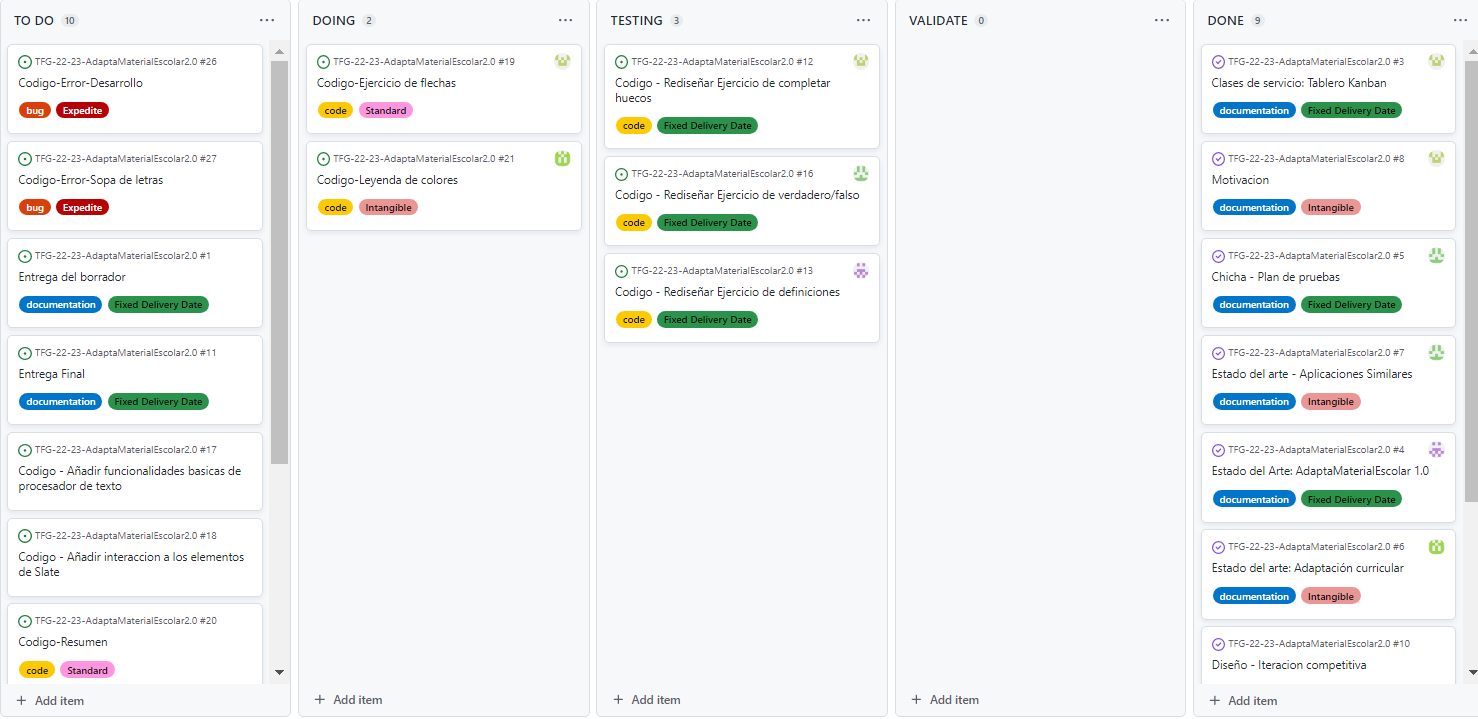
\includegraphics[width=0.8\textwidth]{Tablero/25-02-2023.PNG}
    \caption{Tablero Kanban 25-02-2023.}
    \label{fig:tabFeb}
  \end{subfigure}

  \begin{subfigure}{\textwidth}
    \centering
    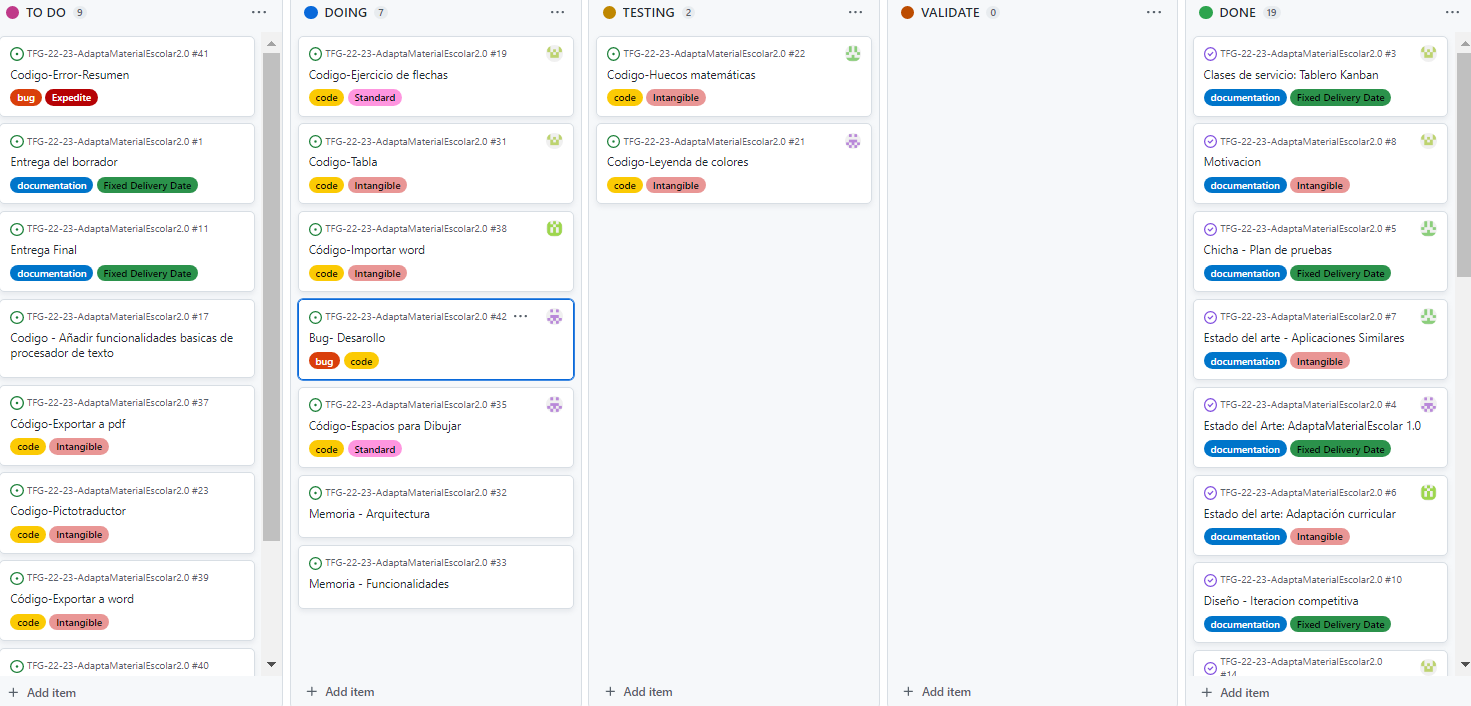
\includegraphics[width=0.8\textwidth]{Tablero/27-03-2023.PNG}
    \caption{Tablero Kanban 27-03-2023.}
    \label{fig:tabmarzo}
  \end{subfigure}

  \begin{subfigure}{\textwidth}
    \centering
    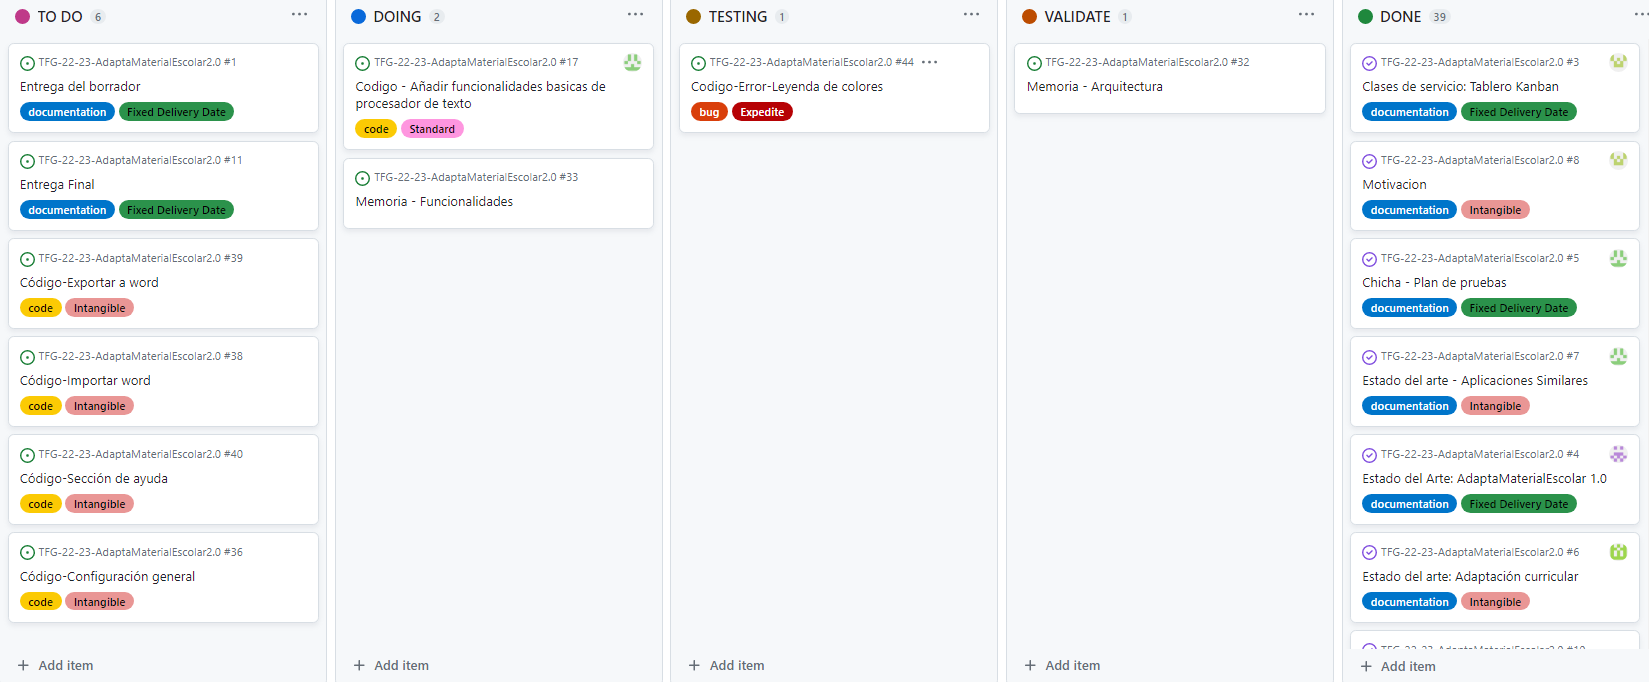
\includegraphics[width=0.8\textwidth]{Tablero/4-05-2023.PNG}
    \caption{Tablero Kanban 4-05-2023.}
    \label{fig:tabmayo}
  \end{subfigure}

  \caption{Tablero Kanban.}
  \label{fig:taleros}
\end{figure}

\subsection{Políticas explícitas}
\label{sec:politicas}
A continuación se presentan las políticas explicitas que hemos ido estableciendo a lo largo del proyecto:

\begin{itemize}
  \item Límites del trabajo en curso (WIP): en las columnas de \textit{Doing} y \textit{Testing} habrá como máximo 2 tareas por persona en cada columna, es decir, no podrá haber más de 8 tareas en cada una de esas columnas.
  \item Definición de \textit{Done}:
        \begin{itemize}
          \item Tareas de memoria: Cuando hayan sido validadas por las tutoras.
          \item Tareas de implementación: Cuando hayan pasado todo el plan de pruebas.
        \end{itemize}
  \item Cuando un integrante del grupo haya terminado su tarea él será el encargado de moverla a la columna correspondiente.
  \item Cualquier integrante del grupo puede poner una tarea en el tablero tras consultarlo con el resto.
  \item Todos los domingos a las 12:00 habrá reunión de equipo para poner en común el trabajo realizado por cada miembro.
  \item Se realizará una reunión de todos los integrantes una semana antes de la revisión con las tutoras para comprobar el trabajo realizado por cada miembro del equipo.
\end{itemize}

\subsection{Clases de servicios}
\label{claseDeServicio}
En Kanban para priorizar las tareas del tablero en ocasiones se emplean las clases de servicio. Estas son una serie de categorías que nos son útiles para clasificar cada una de las tareas de nuestro sistema, las cuales nos permiten identificar rápidamente el nivel de prioridad que tiene la tarea sin hacer un análisis o estimación muy extensa del mismo. Además, la categoría asociada a una tarea determinará como se desplazará la tarea en el tablero. En nuestro caso las clases de servicio que empleamos son las siguientes:
\begin{itemize}
  \item Expedite: Tareas que necesitan ser gestionadas de manera acelerada o urgente. Por ejemplo, algún problema con el editor que nos impediría implementar cualquier otra tarea hasta que esta esté terminada.
  \item Fixed Delivery Date: Tareas con fecha fija que debemos cumplir. Por ejemplo, la corrección de la documentación para la siguiente reunión con las tutoras.
  \item Standard: Tareas que ya ha hecho antes el equipo que no tienen una fecha fija y que ya saben cómo realizar. Por ejemplo, la realización de pruebas de control de calidad de rutina en el software.
  \item Intangible: Tareas que son nuevas para el equipo, tareas que nunca antes han realizado y por tanto, se desconoce el tiempo que se le va a dedicar y el riesgo que suponen. Por ejemplo, la función de exportar a PDF.
\end{itemize}

Para su aplicación tomaremos unas medidas en base a su prioridad. Las clases \textit{Expedite} son las más prioritarias por lo que serán las primeras en ser realizadas. Las \textit{Fixed Delivery Date} serán las siguientes, si en su debida fecha (la cual estará indicada en su descripción) no están implementadas, se convierten en \textit{Expedite} (pasaran a ser más prioritarias). Las \textit{Standard} son un poco menos prioritarias que las \textit{Fixed Delivery Date} al contar con el coste y el esfuerzo que suponen pero presentan un cierto grado de incertidumbre al no tener una fecha fija. Por último, se elegirán las \textit{Intangibles} su prioridad varía al presentar un alto grado de incertidumbre, ya que inicialmente se desconoce el riesgo que suponen pero pueden convertirse en \textit{Standard} o en \textit{Expedite}.

\section{Aseguramiento de la Calidad (QA)}\label{sec:qa}
En esta sección se explican las medidas que se han tomado en el proyecto para asegurar la calidad del software. La importancia de un formato consistente y limpio del código fuente se explica en la Sección \ref{sec:qaformato}, el uso de la técnica de análisis linting para detectar errores antes de la ejecución de la aplicación se cuenta en la Sección \ref{sec:qalinting} y el plan de pruebas que se ha seguido en el proyecto para asegurar el correcto funcionamiento de la aplicación está en la Sección \ref{sec:qapruebas}.

\subsection{Formato del código}\label{sec:qaformato}
Cuando varios desarrolladores trabajan en un proyecto, es común que tengan diferentes estilos de escritura de código, lo que puede dificultar la lectura y el mantenimiento de este. Para mejorar la calidad del código se ha decidido utilizar una herramienta para dar formato al código. Esta herramienta permite mantener un estilo consistente y limpio, facilitando la lectura del código escrito por otros miembros del equipo ya que no es necesario habituarse al estilo de cada uno. Para ello vamos a utilizar la herramienta Prettier explicada en la Sección \ref{sec:prettier}.

\subsection{Linting}\label{sec:qalinting}
El linting es una técnica de análisis estático de código que busca errores de programación, inconsistencias y malas prácticas en el código fuente. En otras palabras, es una técnica de control de calidad que ayuda a los desarrolladores a identificar y corregir errores en su código antes de que sea utilizado en producción. Con el uso del Linting se pueden detectar errores de sintaxis, ``malas prácticas'' y código poco intuitivo o difícil de mantener. Con este fin hemos usado en el proyecto la herramienta ESLint explicada en la Sección \ref{sec:eslint}.

\subsection{Plan de Pruebas}\label{sec:qapruebas}
Para asegurar el correcto funcionamiento del software construido se ha decidido realizar pruebas manuales, ya que se ha considerado que para el tamaño actual del proyecto no supone un problema realizar pruebas manuales para comprobar las distintas funcionalidades. Si, en un futuro, se decide extender la aplicación y añadir más funcionalidades es recomendable actualizar este plan de pruebas, incluyendo pruebas automatizadas e integración continua. Las pruebas de una tarea de implementación concreta las realizará algún miembro del equipo que no haya participado en el desarrollo de esta y las hará cuando la tarea se encuentre en la columna de \textit{Testing}. La ventaja de que las pruebas las realice un miembro que no se haya visto involucrado en el desarrollo de la tarea es que puede sacar más casos de prueba que aquellos miembros que han implementado la tarea y conocen el código.

Cuando un miembro del equipo se haya asignado una tarea de implementación para probar, tendrá que seguir los siguientes pasos:
\begin{enumerate}
  \item \textbf{Generación de los casos de prueba}: Se realizará una tabla con los distintos casos de prueba que se utilizarán para probar una funcionalidad concreta, teniendo en cuenta los requisitos de usuario. Los casos de prueba se entienden como las condiciones de ejecución (precondiciones), el conjunto de entradas, el objetivo de la prueba (campos y condiciones que se quieren comprobar) y los resultados esperados tras ejecutar la prueba (postcondiciones). En la Tabla \ref{tab:ejemplocasosprueba} se muestra un ejemplo de los casos de prueba utilizados en el proyecto.
  \item \textbf{Definición de los procedimientos de la prueba}: Después de generar los casos de prueba, se definirá un guion en el que se explicarán los pasos a seguir para la ejecutar la prueba. En este guion se deben tener en cuenta todos los casos de prueba generados anteriormente. Cada paso debe ser claro y concreto, además de ofrecer ejemplos de datos de entrada, por ejemplo ``Escribir `hola'\, en el campo de añadir frase.'' o ``Pulsar botón de añadir frase.''.
  \item \textbf{Ejecución de la prueba}: Una vez se hayan definido los pasos necesarios para probar una funcionalidad concreta, hay que ejecutar la prueba, siguiendo estos pasos. Durante la ejecución, se registrarán los resultados obtenidos que no concuerden con los resultados esperados o comportamientos de la funcionalidad que puedan afectar negativamente a la experiencia de usuario.
  \item \textbf{Realización del informe de prueba}: Finalmente, en caso de que al realizar la prueba se hayan encontrado fallos, se deberá crear una incidencia de tipo \textit{bug} con la clase de servicio \textit{Expedite}. En la descripción de esta incidencia se deberá informar de los resultados obtenidos, los resultados esperados y los pasos a seguir para replicar cada fallo o problema que haya ocurrido durante la ejecución de la prueba. También se puede incluir información que pueda ser relevante para encontrar una solución a cada fallo o problema. En la Figura \ref{fig:ejemploerrores} se muestra un ejemplo de una incidencia con los errores encontrados tras ejecutar el plan de pruebas. En caso de no haber encontrado errores, se cerrará la incidencia del desarrollo de la funcionalidad que se está probando.
\end{enumerate}

\begin{table}[H]
  \resizebox{1\textwidth}{!}{
    \begin{tabular}{|c|c|c|c|c|}
      \hline
      \textbf{Precondición}       & \textbf{Campo}   & \textbf{Condición}                                             & \textbf{Datos de entrada}   & \textbf{\begin{tabular}[c]{@{}c@{}}Salida esperada\\ (Postcondición)\end{tabular}} \\ \hline
      Lista={[} {]}               & Nueva frase      & Longitud de frase \textless{}= 0                               & Frase = “”                  & Lista = {[} {]}                                                                    \\ \hline
      Lista={[} {]}               & Nueva frase      & Longitud de frase \textgreater 0                               & Frase = “hola”              & Lista = {[}“hola” {]}                                                              \\ \hline
      Lista={[}“hola”{]}          & Editar frase     & Longitud de frase \textless{}= 0 y la Frase existe en la lista & Frase = “”                  & Lista = {[}“hola”{]}                                                               \\ \hline
      Lista={[}“hola”{]}          & Editar frase     & Longitud de frase \textgreater 0 y la Frase existe en la lista & Frase = “adios”             & Lista = {[}“adios”{]}                                                              \\ \hline
      Lista={[}“hola”{]}          & Borrar frase     & Existe la frase a borrar en la lista                           & Frase = “hola”              & Lista = {[} {]}                                                                    \\ \hline
      Lista={[}“hola”, “adios”{]} & Reordenar frases &                                                                & Lista={[}“hola”, “adios”{]} & Lista = {[}“adios”, “hola”{]}                                                      \\ \hline
      Lista={[}{]}                & Reordenar frases &                                                                & Lista={[}{]}                & Lista={[}{]}                                                                       \\ \hline
      Lista={[}“hola”{]}          & Reordenar frases &                                                                & Lista={[}“hola”{]}          & Lista={[}“hola”{]}                                                                 \\ \hline
    \end{tabular}
  }
  \caption{Ejemplo de casos de prueba (Funcionalidad verdadero/falso).}
  \label{tab:ejemplocasosprueba}
\end{table}

\begin{figure}[ht!]
  \centering
  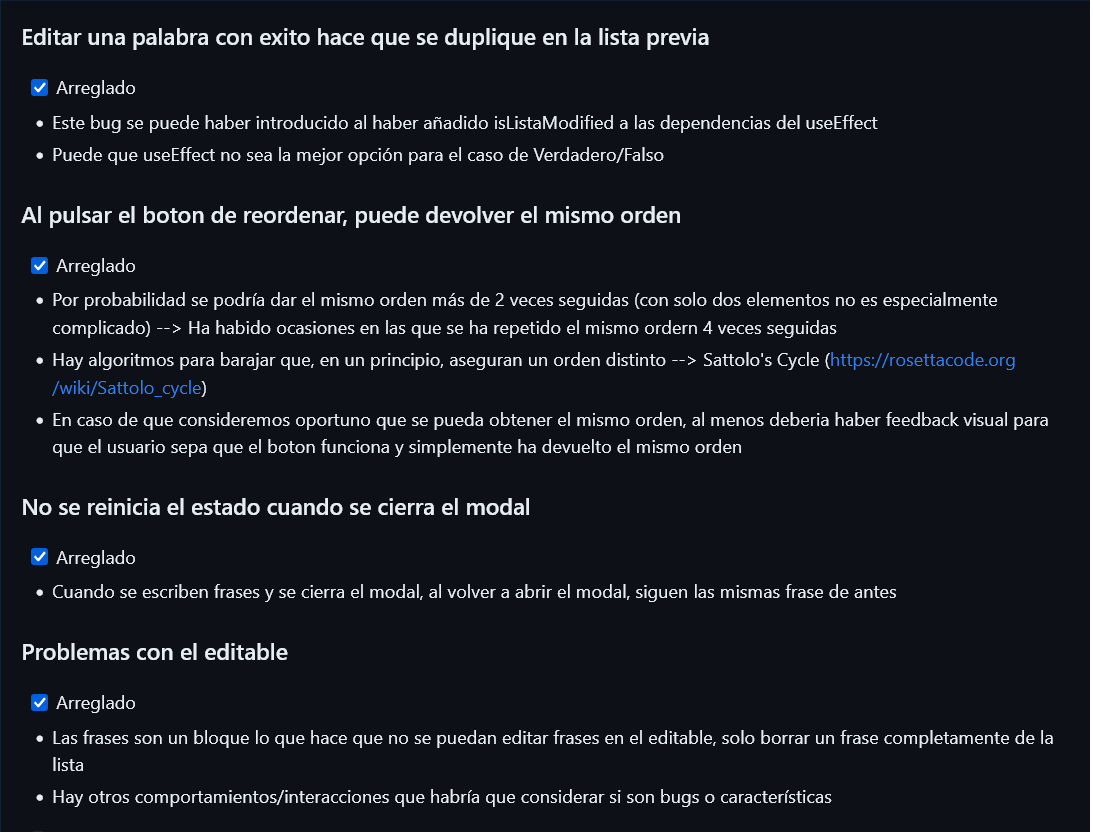
\includegraphics[width=1\textwidth]{QA/ErroresVF.png}
  \caption{Incidencia de errores (Funcionalidad verdadero/falso).}
  \label{fig:ejemploerrores}
\end{figure}

Los casos de prueba, guiones de prueba y errores encontrados de cada funcionalidad se muestran en el Apéndice \ref{ape:pruebas}.